% Stanford University PhD thesis style -- modifications to the report style
% This is unofficial so you should always double check against the
% Registrar's office rules
% See http://library.stanford.edu/research/bibliography-management/latex-and-bibtex
% 
% Example of use below
% See the suthesis-2e.sty file for documentation
%
\documentclass[12pt]{report}
\usepackage{suthesis-2e}  % (modified) Stanford thesis style file

% useful packages
\usepackage{graphicx}  % figures
\usepackage{textcomp}  % load before gemsymb to suppress ``Not defining {\pertthousand / \micro}'' warnings
\usepackage{gensymb}  % \degree
\usepackage{siunitx}  % SI units
\usepackage{tabularx}  % nice single page tables
\usepackage{longtable}  % tables spanning multiple pages
\usepackage{hyperref}  % URLs
\usepackage[english]{babel}  % load before csquotes to suppose ``No multilingual support'' warning
\usepackage[autostyle,english=american]{csquotes}  % quote orientation
\MakeOuterQuote{"}

% use png first, otherwise pdf
% (useful for faster compile times, for final submission switch order)
\DeclareGraphicsExtensions{.png,.pdf}

\begin{document}
\title{How to Write Theses\\
            With Two Line Titles}
\author{Your name}
\dept{Your department}
\principaladvisor{Professor name 1}
\firstreader{Professor name 2}
\secondreader{Professor name 3}
% \thirdreader{Jane Supernumerary}  % uncomment if needed
% \fourthreader{Severus Snape}  % uncomment if needed
 
% no signature or copyright pages in online submission
% (they are added by the library)

% including chapters, no .tex extension necessary
\beforepreface
\documentclass[../main.tex]{subfiles}
\begin{document}

\prefacesection{Abstract}

My abstract.

\ifSubfilesClassLoaded{\bibliography{../mybib}}{}
\end{document}

\documentclass[../main.tex]{subfiles}
\begin{document}

\prefacesection{Acknowledgements}

I would like to thank...

\ifSubfilesClassLoaded{\bibliography{../mybib}}{}
\end{document}

\afterpreface
\documentclass[main.tex]{subfiles}
\begin{document}

\chapter{Introduction}

\section{Background}
Broad overview.

\subsection{Specific background}
Specific text.

\end{document}

\documentclass[main.tex]{subfiles}
\begin{document}

% Full title as you would like it to appear on the page
\chapter{Long paper 1 chapter title}
% Short title that appears in the header of pages within the chapter
\chaptermark{Short chapter title}

\section{Abstract}
Concise introduction, motivation, results, and conclusions.

\section{Introduction}
Examples of citations: we knew X from \cite{Croote201616022} and Y from \cite{Croote20181306}.

\section{Results}
\subsection{Result 1}
Here is a reference to Figure \ref{fig:paper1_fig1}.
We found bacteria, roughly 5 \si{\mu}m in length, that live at 95\degree C for roughly 90\% of the year. More symbols: \$, \#, 10\textsuperscript{5}, $\alpha$, $\beta$, $\gamma$, $\kappa$, \textbf{bold}, \textit{italics}.
Quotation marks are "correctly oriented" thanks to the csquotes package.
Now an inline equation: $E = mc^2$. Now a reference to Equation \ref{eqn:paper1_eqn1}:
\begin{equation}\label{eqn:paper1_eqn1}
d_t = \frac{c - pn_t}{n_t}
\end{equation}

\begin{figure}[hbt!]
\centering
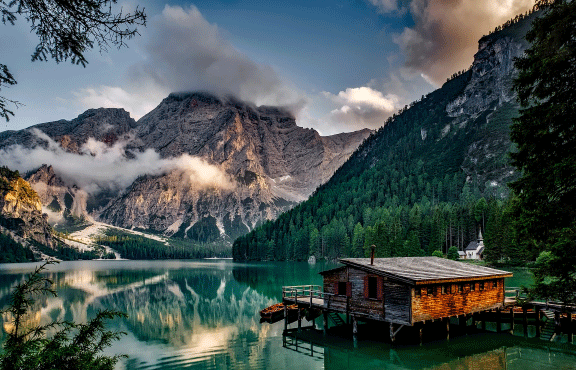
\includegraphics[width=14cm, keepaspectratio]{paper1/fig1.png}
\caption[Short figure caption for List of Figures]{Long figure caption text that explains everything.}
\label{fig:paper1_fig1}
\end{figure}

There will be more text here.

More text here.

More text here.

More text here.

More text here.

More text here.

\subsection{Result 2}
We discovered something else. Here is a reference to Table \ref{tab:paper1_tab1}.

\renewcommand{\arraystretch}{2}  % make spacing nicer
\begin{table}[hbt!]
\centering
\begin{tabularx}{\textwidth}{c|c|c|c}  % 4 columns center-justified
   \textbf{Col 1} & \textbf{Col 2} & \textbf{Col 3} & \textbf{Col 4} \\
   \hline  % horizontal line
   Text in Row 1a & Text in Row 1b & Text in Row 1c & Lots of text in Row 1d \\
                  & Row 1.5b & Row 1.5c & Row 1.5d \\
   \hline
   Row 2a & Row 2b & Row 2c & Row 2d \\
   \hline
   Row 3a & Row 3b & Row 3c & Row 3d \\
\end{tabularx}
\caption[Short table caption for List of Tables]{Long table caption explaining everything.}
\label{tab:paper1_tab1}
\end{table}

More text here.

More text here.

More text here.

More text here.

\begin{sloppypar}
FixAwkwardSpacingWithSloppypar FixAwkwardSpacingWithSloppypar FixAwkwardSpacingWithSloppypar FixAwkwardSpacingWithSloppypar FixAwkwardSpacingWithSloppypar.
\end{sloppypar}

More text here.

More text here.

\section{Conclusions}
The end of the paper.

% Uncomment to print the bibliography when compiling individual chapters
\iftoggle{biblatex}{
  \ifSubfilesClassLoaded{\printbibliography}{}
}{
  \ifSubfilesClassLoaded{\bibliography{../bib/mybib}}{}
}
\end{document}

\documentclass[main.tex]{subfiles}
\begin{document}

\chapter{Concluding Remarks}

I conclude...

\end{document}


% uncomment below if you have an appendix
% \appendix
% \chapter{A Long Proof}

\bibliographystyle{unsrt}  % can change to fit your field e.g. pnas2009
\bibliography{mybib}  % no .bib extension necessary

% adds a non-numbered signature page at end (for printing on ACID-FREE paper)
% (remember to comment out when submitting final version)
\onlinesignature

\end{document}
